% !TeX encoding=utf8
% !TeX spellcheck = de_CH_frami

\chapter{Einleitung}
Im Rahmen der Bachelorarbeit werden Buchungsdaten von Interhome analysiert, um daraus Erkenntnisse zu gewinnen. In der Einleitung wird die Aufgabenstellung erläutert, sowie Abgrenzungen definiert.
 
\section{Aufgabenstellung}
Nachfolgend ist die Aufgabenstellung aufgeführt, wie sie für die Projektfreigabe eingereicht wurde.

\subsection{Ausgangslage}
Interhome AG vertreibt Ferienwohnungen auf einer Webseite mit 26 Domains und 14 Sprachen, welche mit dem Content Management System Sitecore umgesetzt ist. Darauf können Kunden Ferienhäuser oder -wohnungen (Objekte) buchen. Zuerst muss der User eine Destination auswählen und kann dann die verschiedenen Objekte ansehen. Diese haben einen Namen, Bilder und 18 dargestellte Attribute. Beispiele solcher Attribute sind, ob die Wohnung einen Fernseher besitzt, Tiere erlaubt sind oder eine Sauna vorhanden ist. Dies sind binäre Werte, welche wahr oder falsch sein können. Es gibt zusätzlich noch kontinuierliche Attribute wie Distanz um Meer oder zum Zentrum.

Die Buchungen werden in das \gls{irent} gespeichert. Die gesammelten Daten werden von einem Recommender System, welches von Interhome entwickelt wurde, analysiert. Weitere Untersuchungen der Daten finden im Moment nicht statt.

\subsection{Ziel der Arbeit}
Das Ziel der Arbeit ist es, Interhome eine Plattform zur Verfügung zu stellen, damit neue Informationen aus den Buchungsdaten extrahiert werden können (Knowledge Discovery). Dafür wird entweder ein bestehendes Programm verwendet oder eine eigene Lösung entwickelt. Es soll möglich sein, zum Beispiel eine folgende Frage zu beantworten: „Was für Objekte werden im Winter am meisten in Zermatt gebucht?“. Eine mögliche Antwort wäre: „Objekte welche unter CHF500 kosten und maximal 200 Meter von einem Skilift entfernt sind“.
Dies sollte Interhome ermöglichen, ihre Marketing Strategie zu verbessern und gezielter Objekte einzukaufen.

Um solche Fragen zu beantworten werden die Buchungsdaten von Interhome (Objekt, Zeitraum, Passagiere, etc.) ausgelesen (ca. 1-2 Millionen) und mit weiteren Daten (Objektattribute, Geolocation und Wetterinformation) angereicht. 
Auf dem Endprodukt soll ein Mitarbeiter von Interhome in der Lage sein, ein Abfrage zu generieren, welche aus einem oder mehreren Attribute besteht. Die Applikation analysiert daraufhin die Daten mit Techniken des Data Mining, um eine Liste von Attributen zurück zu liefern, welche für die in der Abfrage aufgeführten Attributen am meisten Buchungen generieren. Die Elemente in der Antwort sollten gewichtet sein um das Resultat besser zu interpretieren.

Die Daten können schlussendlich weiterverwendet werden, um gezielter Werbung an die Kunden zu bringen. Es sollte möglich sein, personalisierte Werbung zu schalten. Wenn ein Kunde aus dem Grossraum Zürich die Webseite bucht, können Objekte angezeigt werden welche von Personen aus dieser Region am meisten gebucht wird. 

\section{Abgrenzung}
Dieses Kapitel beschreibt sämtliche Projektabgrenzungen, welche für dieses Projekt definiert
wurden.

\subsection{Zeitliche Abgrenzung}
Für diese Arbeiten geltet die zeitliche Vorgabe der \gls{zhaw} von 6 Monaten mit einem Arbeitsaufwand von 360 Stunden.
Der Start der Arbeit beginnt mit der Abnahme der Aufgabenstellung, welche am 04.11.2016 stattfand.
Demnach endet die Arbeit am 04.05.2017.

\subsection{Sachliche Abgrenzung}
Ziel der Arbeit ist es, eine Plattform zu schaffen auf welcher die Buchungsdaten von Interhome exploriert werden können. Dazu müssen die Daten aus dem Irent extrahiert und mit Techniken des Data Mining analysiert werden. Schlussendlich wird das Resultat bewertet, sodass entschieden werden kann ob es sich für einen produktiven Einsatz eignet.

Nicht beinhaltet in der Arbeit ist die Verbesserung der Marketing Strategie. Dies sollte durch das Projekt ermöglicht werden, ist jedoch nicht teil davon. Zusätzlich könnte die Plattform nützlich sein, um personalisierte Werbung auf der Webseite von Interhome zu schalten. Dies ist jedoch auch nicht im Umfang der Arbeit enthalten.

\subsection{Projektbeteiligte}
\begin{table}[H] 
	\caption{Projektbeteiligte}
	\centering
	\rowcolors{1}{tablebodycolor}{tablerowcolor}
	
	\begin{tabular}{ | c | c | c | c |} 
		\hline 
		\rowcolor{tableheadcolor}
		\bfseries Beschreibung & 
		\bfseries Firma/Institution & 
		\bfseries Personen \\ \hline 
		Auftraggeber & Hotelplan Management AG & Christian Kiser \\ \hline 
		Projektleitung & Hotelplan Management AG & Simon Lang\\ \hline 
		Projektbetreuerin &  \gls{zhaw} & Dr. Ruxandra Domenig \\ \hline 
		Experte & \gls{zhaw} & Christioph Burkhardt \\ \hline 
	\end{tabular} 
\end{table}

\section{Vorgehen}
Nachfolged wird das Vorgehen für die Analyse der Daten und die Umsetzung des Prototypen beschrieben.

Zuerst wird in der Recherche (siehe \cref{sec:recherche} \nameref{sec:recherche}) die Daten beschafft, welche im Rahmen dieser Arbeit zu untersuchen sind. Für das Data Mining werden verschiedene Techniken aufgeführt, welche sich für die Analyse eignen könnten. Zusätzlich werden noch existierende wissenschaftliche Arbeiten gesucht welche sich mit derselben Thematik auseinandersetzen. Zum Abschluss werden noch Programme evaluiert, welche für das Data Mining eingesetzt werden können.

Das zweite Kapitel widmet sich der Anforderungsanalyse (siehe \cref{sec:anforderungsanalyse} \nameref{sec:anforderungsanalyse}). Darin werden die Anforderungen an die Data Mining Techniken beschrieben, welche im Kapitel Recherche erläutert wurden. Zusätzlich werden Die Buchungsdaten analysiert und zuletzt die Voraussetzungen definiert, welche die Plattform für das Knowledge Discovery zu erfüllen hat.

Nachdem die Anforderungen festgelegt wurden wird ein Konzept (siehe \cref{sec:konzept} \nameref{sec:konzept}) erstellt. Dieses legt fest, welche Data Mining Techniken in der Arbeit verwendet werden. Zusätzlich werden folgende Punkte im Bezug an die Platform für das Knowledge Discovery definiert:
\begin{itemize}
	\item Wird ein bestehendes Programm verwendet oder eine eigene Implementation.
	\item Design und Funktionalität der Plattform.
	\item Testcases der Plattform.
\end{itemize}

Anschliessend startet das Proof of Concept (siehe \cref{sec:proofofconcept} \nameref{sec:proofofconcept}). Darin müssen zuerst die Daten für die Analyse vorbereitet werden. Danach wird die Plattform aufgesetzt oder implementiert.

Zum Abschluss werden die Testcases aus dem Konzept ausgewertet und ein Fazit gezogen.

\section{Grobplanung}
In der \cref{fig:einleitung:projektablaufplan} \nameref{fig:einleitung:projektablaufplan} ist der Projektablaufplan dargestellt.
\begin{sidewaysfigure}[h]
	\centering
	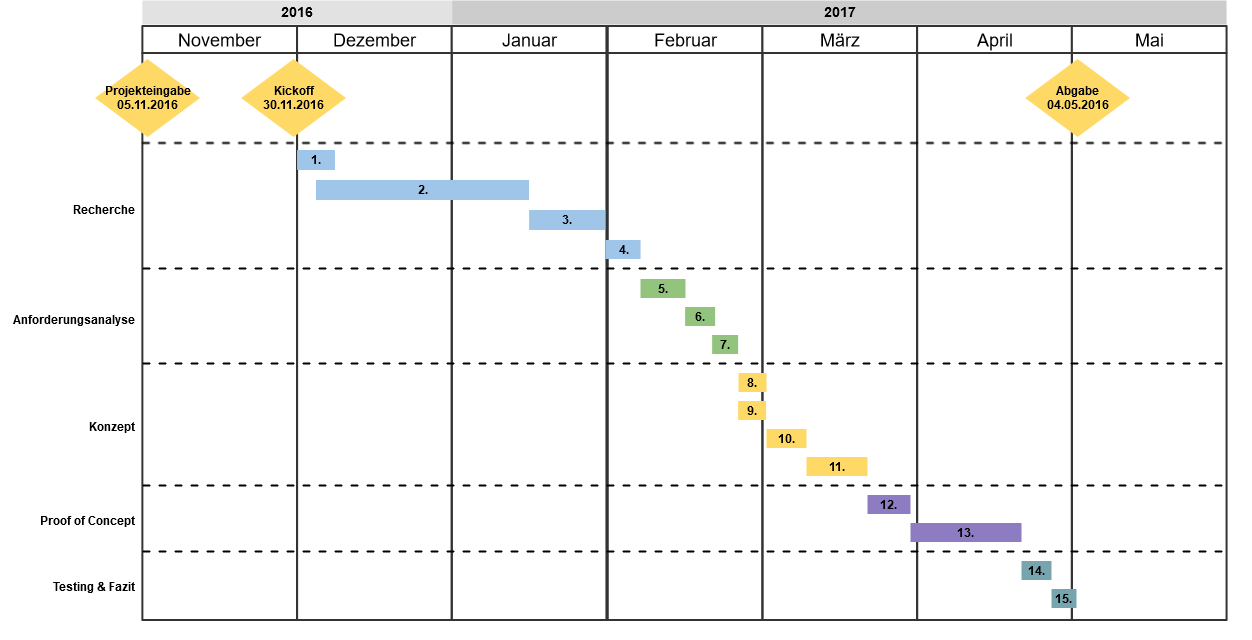
\includegraphics[width=1\textwidth]{images/projektablaufplan.png}
	\caption{Projektablaufplan}
	\label{fig:einleitung:projektablaufplan}
\end{sidewaysfigure}
\\\\
{\parindent0pt % disables indentation for all the text between { and }
Nachfolgend die Beschreibung der einzelnen Arbeitsschritte des Projektplanes.\\

Recherche:\\
1. Beschaffung der Buchungsdaten für die Auswertung.\\
2. Evaluation von verschiedenen Techniken des Data Mining, welche für die Auswertung der Daten verwendet werden können.\\
3. Vorhandene wissenschaftliche Arbeiten suchen, welche sich mit einer ähnlichen Problemstellung auseinandersetzen.\\
4. Evaluation von verschiedenen Programmen für die Auswertung und Darstellung der Daten.\\

Anforderungsanalyse:\\
5. Beschreibung der Vorgehensweisen, welche in wissenschaftlichen Arbeiten gefunden wurden und sich für die Problemstellung eignen. \\
6. Analyse der Buchungsdaten für die Auswertung.\\
7. Anforderungen an das Programm für die Auswertung und Darstellung der Daten.\\

Konzept:\\
8. Definition einer Vorgehensweise für die Datenanalyse.\\
9. Festlegen ob ein Programm für die Auswertung und Darstellung der Daten verwendet wird oder eine eigene Implementation.\\
10. Design und Funktionalität des Programmes definieren.\\
11. Definition der Testcases an das Programm.\\

Proof of Concept:\\
12. Vorbereitung der Daten für die Auswertung.\\
13. Erstellung oder Verwendung eines Programmes für die Analyse und Darstellung der Daten.\\

Testing \& Fazit\\
14. Auswertung der Testcases.\\
15. Einschätzung ob das Programm live für Interhome eingesetzt werden kann.
}